\documentclass[12pt]{beamer}
\newenvironment{ConCodigo}[1]
  {\begin{frame}[fragile,environment=ConCodigo]{#1}}
  {\end{frame}}
\graphicspath{{Imagenes/}{../Imagenes/}}
\usepackage[utf8]{inputenc}
\usepackage[spanish]{babel}
\usepackage{hyperref}
\usepackage{etex}
%\reserveinserts{28}
\usepackage{amsmath}
\usepackage{amsthm}
\usepackage{mathtools}
\usepackage{multicol}
\usepackage{multirow}
\usepackage{tabulary}
\usepackage{booktabs}
\usepackage{nccmath}
\usepackage{physics}
\usepackage{biblatex}
\usepackage[outdir=./]{epstopdf}
%\epstopdfsetup{outdir=./}
\usepackage{graphicx}
%\usepackage{enumitem,xcolor}
\usepackage{siunitx}
%\sisetup{scientific-notation=true}
%\usepackage{fontspec}
\usepackage{lmodern}
\usepackage{float}
\usepackage[format=hang, font=footnotesize, labelformat=parens]{caption}
\usepackage[autostyle,spanish=mexican]{csquotes}
\usepackage{standalone}
\usepackage{blkarray}
\usepackage{algorithm}
\usepackage{algorithmic}
\usepackage{tikz}
\usepackage[siunitx, RPvoltages]{circuitikz}
\usetikzlibrary{arrows,patterns,shapes}
\usetikzlibrary{decorations.markings}
\usetikzlibrary{arrows}
\usepackage{color}
\usepackage{xcolor}
%\usepackage{beton}
%\usepackage{euler}
%\usepackage[T1]{fontenc}
\usepackage[sfdefault]{roboto}  %% Option 'sfdefault' only if the base font of the document is to be sans serif
\usepackage[T1]{fontenc}
\renewcommand*\familydefault{\sfdefault}
\DeclareGraphicsExtensions{.pdf,.png,.jpg}
\usepackage{hyperref}
\renewcommand {\arraystretch}{1.5}
\newcommand{\python}{\texttt{python}}
\usefonttheme[onlymath]{serif}
\setbeamertemplate{navigation symbols}{}
\usetikzlibrary{patterns}
\usetikzlibrary{decorations.markings}
\tikzstyle{every picture}+=[remember picture,baseline]
%\tikzstyle{every node}+=[inner sep=0pt,anchor=base,
%minimum width=2.2cm,align=center,text depth=.15ex,outer sep=1.5pt]
%\tikzstyle{every path}+=[thick, rounded corners]
\setbeamertemplate{caption}[numbered]
\newcommand{\ptm}{\fontfamily{ptm}\selectfont}
%Se usa la plantilla Warsaw modificada con spruce
\mode<presentation>
{
  \usetheme{Warsaw}
  \setbeamertemplate{headline}{}
  \useoutertheme{default}
  \usecolortheme{albatross}
  \setbeamercovered{invisible}
}
% \AtBeginSection[]
% {
% \begin{frame}<beamer>{Contenido}
% \normalfont\mdseries
% \tableofcontents[currentsection]
% \end{frame}
% }

\input{../Preambulos/pre_plantilla_Warsaw_spruce}
\input{../Preambulos/pre_codigo}
\makeatletter
\setbeamercolor{section in foot}{bg=gray!30, fg=black!90!orange}
\setbeamercolor{subsection in foot}{bg=blue!30!yellow, fg=red}
\setbeamertemplate{footline}
{
  \leavevmode%
  \hbox{%
  \begin{beamercolorbox}[wd=.333333\paperwidth,ht=2.25ex,dp=1ex,center]{section in foot}%
    \usebeamerfont{section in foot} \insertsection
  \end{beamercolorbox}}%
  \begin{beamercolorbox}[wd=.333333\paperwidth,ht=2.25ex,dp=1ex,center]{subsection in foot}%
    \usebeamerfont{subsection in foot}  \insertsubsection
  \end{beamercolorbox}%
  \begin{beamercolorbox}[wd=.333333\paperwidth,ht=2.25ex,dp=1ex,right]{date in head/foot}%
    \usebeamerfont{date in head/foot} \insertshortdate{} \hspace*{2em}
    \insertframenumber{} / \inserttotalframenumber \hspace*{2ex} 
  \end{beamercolorbox}}%
  \vskip0pt%
\makeatother
\title{\large{Tema 2 - Operaciones matemáticas básicas}}
\subtitle{Técnicas de Interpolación II}
\author{M. en C. Gustavo Contreras Mayén}
\date{\today}
\institute{Facultad de Ciencias - UNAM}
\titlegraphic{\includegraphics[width=1.75cm]{Imagenes/escudo-facultad-ciencias}\hspace*{4.75cm}~%
   \includegraphics[width=1.75cm]{Imagenes/escudo-unam}
}
\begin{document}
\maketitle
\fontsize{14}{14}\selectfont
\spanishdecimal{.}
\section*{Contenido}
\frame{\tableofcontents[currentsection, hideallsubsections]}
\section{Métodos polinomiales}
\frame{\tableofcontents[currentsection, hideothersubsections]}
\begin{frame}
\frametitle{Técnicas de interpolación}
Continuamos revisando algunas técnicas de inteporlación de datos.
\end{frame}
\subsection{Interpolación de Newton}
\begin{frame}
\frametitle{Interpolación de Newton}
Aunque el método de interpolación de Lagrange es conceptualmente sencillo, no es en sí, un algoritmo eficiente.
\\
\medskip
\pause
Un mejor método computacional se obtiene con el Método de Newton, donde el polinomio de interpolación se escribe de la forma:
\begin{align*}
\begin{aligned}
P_{n}(x) = a_{0} + (x &- x_{0}) \: a_{1} + (x - x_{0})(x-x_{1}) \: a_{2} + \ldots + \\
&+ (x - x_{0})(x - x_{1}) \ldots (x - x_{n - 1}) \: a_{n} 
\end{aligned}
\end{align*}
\end{frame}
\begin{frame}
\frametitle{Polinomio de Newton}
Este polinomio nos permite contar con un procedimiento de evaluación más eficiente.
\\
\medskip
Por ejemplo, con cuatro pares de datos ($n = 3$), tenemos que el polinomio de interpolación es:
\begin{align*}
P_{3}(x) &= a_{0} + (x - x_{0}) \: a_{1} + (x - x_{0})(x - x_{1}) \: a_{2} + \\		
&+ (x - x_{0})(x - x_{1})(x - x_{2}) \: a_{3} \\
P_{3}(x) &= a_{0} + \left\lbrace a_{1} + (x - x_{1}) \left[a_{2} + (x - x_{2}) \: a_{3} \right] \right\rbrace 
\end{align*}
que puede ser evaluado hacia atrás con las siguientes relaciones de recurrencia:
\end{frame}
\begin{frame}[fragile]
\frametitle{Relaciones de recurrencia}
\begin{align*}
P_{0} &= a_{3} \\
P_{1} &= a_{2} + (x - x_{2}) \: P_{0}(x) \\
P_{2} &= a_{1} + (x - x_{1}) \: P_{1}(x) \\
P_{3} &= a_{0} + (x - x_{0}) \: P_{2}(x) 
\end{align*}
\pause
Para un $n$ arbitrario, tenemos:
\pause
\begin{align*}
P_{0}(x) &= a_{n} \\
P_{k} &= a_{n - k} + (x - x_{ n - k}) \: P_{k - 1}(x), \hspace{0.5cm} k = 1, 2, \ldots, n
\end{align*}
\end{frame}
\subsection{Construcción del algoritmo}
\begin{frame}[fragile]
\framesubtitle{Construcción del algoritmo}
Definimos \texttt{xDatos} para las coordenadas $x$ del conjunto de puntos y $n$ al grado de polinomio, podemos usar el siguiente algoritmo para calcular el polinomio de Newton $P_{n}(x)$:
\begin{lstlisting}[caption=Cálculo del polinomio de Newton,style= FormattedNumber, basicstyle=\linespread{0.9}\ttfamily=\small, columns=fullflexible]
p = a[n]
for k in range(1, n + 1):
    p = a[n - k] + (x - xDatos[n - k])*p
\end{lstlisting}
\end{frame}
\begin{frame}
\frametitle{Construcción del algoritmo}
Los coeficientes de $P_{n}$ se calculan forzando que el polinomio pase a través del conjunto de puntos
\[ y_{i} = P_{n}(x_{i}),\hspace{0.5cm} i = 0, 1, \ldots ,n \]
\end{frame}
\begin{frame}
\frametitle{Construcción del algoritmo}
De tal manera que tenemos un sistema de ecuaciones simultáneas:
\begin{align*}
y_{0} &= a_{0} \\
y_{1} &= a_{0} + (x_{1} - x_{0}) \: a_{1} \\
y_{2} &= a_{0} + (x_{2} - x_{0}) \: a_{1} + (x_{2} - x_{0})(x_{2} - x_{1}) \: a_{2} \\
\vdots \\
y_{n} &= a_{0} + (x_{n} - x_{0}) \: a_{1} + \ldots + \\
&+ (x_{n} - x_{0})(x_{n} - x_{1}) \ldots (x_{n} - x_{n-1}) \: a_{n}
\end{align*}
\end{frame}
\subsection{Diferencias divididas}
\begin{frame}[fragile]
\frametitle{Diferencias divididas}
Se introducen las diferencias divididas, de la siguiente forma:
\begin{align*}
\nabla y_{i} &= \dfrac{y_{i} - y_{0}}{x_{i} - x_{0}}, \hspace{1cm} i = 1,2,\ldots,n \\
\visible<2->{\nabla^{2} y_{i} &= \dfrac{\nabla y_{i} - \nabla y_{1}}{x_{i} - x_{1}}, \hspace{1cm} i = 1,2,\ldots,n} \\
\visible<3->{\nabla^{3} y_{i} &= \dfrac{\nabla^{2} y_{i} - \nabla^{2} y_{2}}{x_{i} - x_{2}}, \hspace{1cm} i = 1,2,\ldots,n} \\
\visible<4->{\vdots} \\
\visible<5->{\nabla^{n} y_{i} &= \dfrac{\nabla^{n-1} y_{n} - \nabla^{n-1} y_{n-1}}{x_{n} - x_{n-1}}}
\end{align*}
\end{frame}
\begin{frame}
La solución al sistema de ecuaciones es entonce:
\begin{align*}
a_{0} &= y_{0} \\
a_{1} &= \nabla \: y_{1} \\
a_{2} &= \nabla^{2} \: y_{2} \\
\vdots \\
a_{n} &= \nabla^{n} \: y_{n}
\end{align*}
\end{frame}
\begin{frame}
\frametitle{Coeficientes del polinomio}
Si los coeficientes se calculan a mano, es convieniente escribirlos con el siguiente formato:
(con $n = 4$)
\\
\medskip
\begin{center}
\begin{tabular}{| c | c | c | c | c | c |}
\hline $x_{0}$ & $y_{0}$ & & & & \\
\hline $x_{1}$ & $y_{1}$ & $\nabla y_{1}$ & & & \\
\hline $x_{2}$ & $y_{2}$ & $\nabla y_{2}$ & $\nabla^{2} y_{2}$ & &  \\
\hline $x_{3}$ & $y_{3}$ & $\nabla y_{3}$ & $\nabla^{2} y_{3}$ & $\nabla^{3} y_{3}$ &  \\
\hline $x_{4}$ & $y_{4}$ & $\nabla y_{4}$ & $\nabla^{2} y_{4}$ & $\nabla^{3} y_{4}$ & $\nabla^{4} y_{4}$ \\
\hline
\end{tabular}
\end{center}
\end{frame}
\begin{frame}
\frametitle{Coeficientes del polinomio}
Los términos en la diagonal principal
\[ y_{0}, \nabla y_{1}, \nabla^{2} y_{2}, \nabla^{3} y_{3}, \nabla^{4} y_{4} \]
son los coeficientes del polinomio.
\\
\medskip
\pause
Si los puntos de datos se enumeran en un orden diferente, las entradas de la tabla van a cambiar, pero el polinomio resultante será el mismo, recordemos que un polinomio de interpolación de grado $n$ con $n + 1$ datos diferentes, es único.
\end{frame}
\begin{frame}[fragile]
\frametitle{Coeficientes del polinomio}
Las operaciones en la computadora se pueden realizar con un arreglo unidimensional $a$, usando el siguiente algoritmo (tomando la notación $m = n + 1$ = número de puntos):
\\
\medskip
\begin{lstlisting}[caption=Coeficiente del polinomio de Newton, style= FormattedNumber, basicstyle=\linespread{1.1}\ttfamily=\small, columns=fullflexible]
a = yDatos.copy()
for k in range(1, m):
    for i in range(k, m):
        a[i] = (a[i] - a[k-_1_])/(xDatos[i] - xDatos[k-_1_])
\end{lstlisting}
\end{frame}
\begin{frame}
Inicialmente el arreglo $a$ contiene las coordenadas $y$ del conjunto de datos, es decir, la segunda columna de la tabla.
\\
\medskip
\pause
Cada vez que pasa por el bucle externo, se genera la siguiente columna, por lo que se sobre-escriben los elementos de $a$, por tanto, al concluir el bucle, $a$ contiene los elementos de la diagonal, que son los coeficientes del polinomio.
\end{frame}
\subsection{Módulos con \python}
\begin{frame}
\frametitle{Módulos con \python}
Para facilitar el mantenimiento y la lectura los programas demasiado largos pueden dividirse en \textcolor{blue}{módulos}, agrupando elementos relacionados.
\\
\bigskip
Los módulos son entidades que permiten una organización y división lógica de nuestro código. Los archivos son su contrapartida física: cada archivo de \python\ almacenado en disco equivale a un módulo.
\end{frame}
\begin{frame}
\subsection{Funciones para el algoritmo}
\frametitle{Módulo con las funciones}
Este módulo incluye dos funciones que se requieren para la interpolación de Newton: la función \azulfuerte{\texttt{coeficientes}} y la función \azulfuerte{\texttt{evaluaPoli}}.
\end{frame}
\begin{frame}
\frametitle{La función \azulfuerte{\texttt{coeficientes}}}
Dados los conjuntos de puntos en los arreglos \texttt{xDatos} y \texttt{yDatos}, la función \azulfuerte{\texttt{coeficientes}} devuelve el arreglo $a$ con los coeficientes.
\end{frame}
\begin{frame}
\frametitle{La función \azulfuerte{\texttt{evaluaPoli}}}
Una vez que ya conocemos los coeficientes, $P_{n}(x)$ puede evaluarse para cualquier valor de $x$ con la función \azulfuerte{\texttt{evaluaPoli}}.
\end{frame}
\begin{frame}[allowframebreaks,     fragile]
\begin{lstlisting}[caption=Funciones en el módulo \texttt{evalPoli},style= FormattedNumber, basicstyle=\linespread{1.1}\ttfamily=\small, columns=fullflexible]    
def coeficientes(xDatos, yDatos):
    m = len(xDatos) 
    a = yDatos.copy()
    for k in range(1, m):
        a[k:m] = (a[k:m] - a[k-_1_])/(xDatos[k:m] - xDatos[k-_1_])
    return a


def evaluaPoli(a, xDatos, x):
    n = len(xDatos) - 1 
    p = a[n]
    for k in range(1,n+_1_):
        p = a[n-k] + (x - xDatos[n-k]) * p
    return p
\end{lstlisting}
\end{frame}
\subsection{Ejercicio a resolver}
\begin{frame}
\frametitle{Ejemplo}
Los datos que se muestran en la siguiente tabla
\begin{table}[htbp]
\centering \small
\begin{tabulary}{15cm}{c | c | c | c | c | c | c}
$x$ & $0.15$ & $2.30$ & $3.15$ & $4.85$ & $6.25$ & $7.95$ \\
\midrule $y$ & $4.79867$ & $4.49013$ & $4.2243$ & $3.47313$ & $2.66674$ & $1.51909$
\end{tabulary}
\end{table}
Se obtuvieron de la función
\[ f(x) = 4.8 \cos \left( \dfrac{\pi \: x}{20} \right)\]
\end{frame}
\begin{frame}
\frametitle{Ejemplo}
Con ese conjunto de datos, interpola mediante el polinomio de Newton para los puntos
\[ x = 0, 0.5, 1.0, 1.5, \ldots,7.5, 8.0 \]
y compara los resultados con el valor \enquote{exacto} de los valores $y_{i} = f(x_{i})$
\end{frame}
\begin{frame}[fragile]
\frametitle{Solución}
¿Qué necesitamos?
\\
\bigskip
Abriendo un archivo en Spyder 3, llamamos al módulo \texttt{numpy} y también al módulo que contiene las funciones para resolver el polinomio de interpolación:
\begin{lstlisting}[style= FormattedNumber, basicstyle=\linespread{1.1}\ttfamily=\small, columns=fullflexible]
from numpy import *
from newtonPoli import *
\end{lstlisting}
\end{frame}
\begin{frame}[fragile]
\frametitle{Cargando los coeficientes}
Hay que crear los arreglos \texttt{xDatos} y \texttt{yDatos}, el arreglo $a$ se obtiene de la función \azulfuerte{\texttt{coeficientes}} que está dentro del módulo \azulfuerte{\texttt{NewtonPoli}}
\begin{lstlisting}[caption=Datos iniciales, style= FormattedNumber, basicstyle=\linespread{1.1}\ttfamily=\small, columns=fullflexible]
xDatos = array([0.15, 2.3, ..., 7.95])
yDatos = array([4.79867, 4.49013, ..., 1.51909])

a = coeficientes(xDatos, yDatos)
\end{lstlisting}
\end{frame}
\begin{frame}[allowframebreaks, fragile]
\frametitle{Evaluación de los puntos}
La siguiente parte es proporcionar el rango de puntos y mandar llamar la función \azulfuerte{\texttt{evalPoli}}:
\\
\medskip
\begin{lstlisting}[caption= Evaluando los puntos, style= FormattedNumber, basicstyle=\linespread{1.1}\ttfamily=\small, columns=fullflexible]
print ('{:^3} \t {:^7} \t {:^7} \t {:<11}'.format('x', 'yInterpol', 'yExacta', 'Err relativo'))
print ('-'*55)

for x in np.arange(0.0, 8.1, 0.5):
    y = evaluaPoli(a, xDatos, x)
    yExacta = 4.8 * np.cos(np.pi*x/20.0)
    print ('{:1.1f} \t {:1.5f} \t {:1.5f} \t {:1.5E}'.format(x, y, yExacta, abs(yExacta - y)/yExacta*100))
\end{lstlisting}
\end{frame}
\begin{frame}
\frametitle{Solución en la terminal}
\fontsize{12}{12}\selectfont
\renewcommand{\arraystretch}{1.1}%
\begin{center}
\begin{tabular}{l l l l}
x & yInterp & yExacta & Err relativo\\
\multicolumn{4}{l}{----------------------------------------------------------} \\
$0.0$ & $4.80003$ & $4.80000$ & $5.22802E-04$ \\
$0.5$ & $4.78518$ & $4.78520$ & $5.16392E-04$ \\
$1.0$ & $4.74088$ & $4.74090$ & $5.70846E-04$ \\
$1.5$ & $4.66736$ & $4.66738$ & $3.19661E-04$ \\
$2.0$ & $4.56507$ & $4.56507$ & $9.67148E-05$ \\
$2.5$ & $4.43462$ & $4.43462$ & $1.57180E-05$ \\
\vdots \\
$7.0$ & $2.17915$ & $2.17915$ & $3.43797E-04$ \\
$7.5$ & $1.83687$ & $1.83688$ & $6.76648E-04$ \\
$8.0$ & $1.48329$ & $1.48328$ & $2.67576E-04$
\end{tabular}
\end{center}
\end{frame}
\begin{frame}
\frametitle{Graficando la función exacta y los puntos}
\begin{figure}
	\centering
	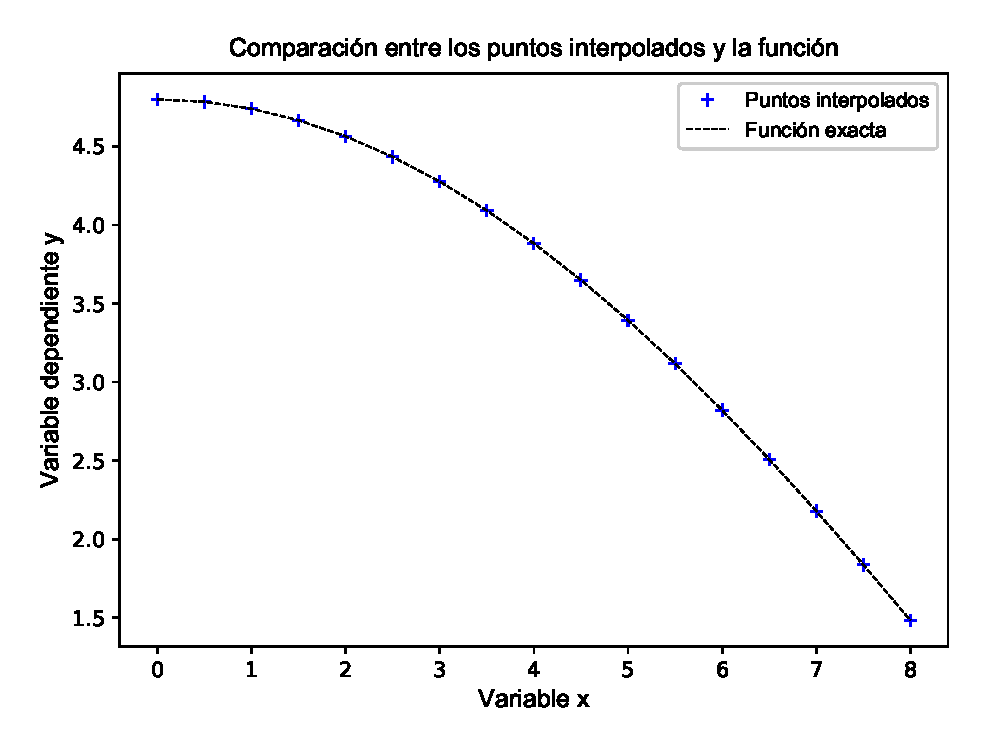
\includegraphics[scale=0.4]{Imagenes/EjemploInterpNewton_01.eps}
    \caption{Los puntos donde se evalúa con el polinomio de Newton, se superponen a la gráfica de la función \enquote{exacta}.}
\end{figure}
\end{frame}
% {
% \setbeamercolor{frametitle}{fg=bisque,bg=ao!90!white}
% \section{Método de Neville}
% \frame{\tableofcontents[currentsection, hideothersubsections]}
% \subsection{Definición del método de Neville}
% \begin{frame}
% \frametitle{Método de Neville}
% Ya vimos que el método de interpolación de Newton consiste en dos pasos:
% \setbeamercolor{item projected}{bg=green!70!black,fg=white}
% \setbeamertemplate{enumerate items}[circle]
% \begin{enumerate}[<+->]
% \item El cálculo de los coeficientes.
% \item La evaluación del polinomio.  
% \end{enumerate}
% \end{frame}
% \begin{frame}
% \frametitle{Método de Neville}
% Esto funciona bien si la interpolación se lleva a cabo repetidamente para diferentes valores de $x$ usando el mismo polinomio. 
% \\
% \bigskip
% Si sólo hay un punto interpolado, el método de Neville es un método que calcula la interpolación en un solo paso, siendo una mejor opción.
% \end{frame}
% \begin{frame}
% \frametitle{Método de Neville}
% Sea 
% \[ P_{k}[x_{i}, x_{i + 1}, x_{i + k}]\]
% el polinomio de orden $k$ que pasa a través de los $k + 1$ pares de puntos:
% \[ (x_{i}, y_{i}), (x_{i + 1}, y_{i + 1}), \ldots, (x_{i+k},y_{i+k}) \]
% \\
% \bigskip
% \pause
% Para un sólo punto, tenemos
% \[ P_{0}[x_{i}] = y_{i}\]
% \end{frame}
% \begin{frame}
% \frametitle{Interpolación de Neville}
% La inteporlación con dos puntos es
% \[ P_{1}[x_{i}, x_{i + 1}] = \dfrac{(x - x_{i + 1}) \: P_{0}[x_{i}] + (x_{i} - x) \: P_{0}[x_{i + 1}]}{x_{i} - x_{i + 1}} \]
% \visible<2->{La inteporlación con tres puntos es}
% \fontsize{12}{12}\selectfont
% \visible<3->{\[ P_{2}[x_{i},x_{i + 1}, x_{i + 2}] = \dfrac{(x - x_{i + 2}) \: P_{1}[x_{i},x_{i + 1}] + (x_{i} - x) \: P_{1}[x_{i + 1}, x_{i + 2}]}{x_{i} - x_{i + 2}} \]}
% \end{frame}
% \begin{frame}
% \frametitle{Interpolación de Neville}
% Para mostrar que esta interpolación intersecta los puntos, sustituimos primero $x = x_{i}$, para obtener
% \[P_{2}[x_{i}, x_{i + 1}, x_{i + 2}] = P_{1}[x_{i}, x_{i + 1}] = y_{i}\]
% \visible<2->{del mismo modo, $x = x_{i + 2}$}
% \visible<3->{\[P_{2}[x_{i}, x_{i + 1}, x_{i + 2}] = P_{1}[x_{i}, x_{i + 2}] = y_{i + 2}\]}
% \visible<4->{finalmente, cuando $x = x_{i + 1}$, tenemos}
% \visible<5->{\[P_{1}[x_{i}, x_{i + 1}] = P_{1}[x_{i + 1}, x_{i + 2}] = y_{i + 1}\]}
% \end{frame}
% \begin{frame}
% \frametitle{Interpolación de Neville}
% Entonces
% \fontsize{12}{12}\selectfont
% \begin{align*}
% P_{2}[x_{i}, x_{i + 1}, x_{i + 2}] = \dfrac{(x_{i + 1} - x_{i + 2}) \: y_{i + 1} + (x_{i} - x_{i + 1}) \: y_{i + 1}}{x_{i} - x_{i + 2}} = y_{i + 1}
% \end{align*}
% \fontsize{14}{14}\selectfont
% Habiendo deducido el patrón, podemos establecer la fórmula recursiva:
% \fontsize{12}{12}\selectfont
% \begin{align*}
% P_{k}[x_{i}, &x_{i + 1},\ldots,x_{i + k}] = \\ 
% &= \dfrac{1}{{x_{i} - x_{i + k}}} \left[ (x - x_{i + k}) \: P_{k - 1}[x_{i}, x_{i + 1}, \ldots, x_{i + k}] + \right. \\
% &+ \left. (x_{i} - x) \: P_{k - 1} [x_{i + 1}, x_{i + 2}, \ldots, x_{i + k}] \right] 
% \end{align*}
% \end{frame}
% \begin{frame}
% \frametitle{Manejando los resultados}
% Dando el valor de $x$, los cálculos se pueden anotar en un formato de tabla (se muestran para cuatro puntos):
% \fontsize{12}{12}\selectfont
% \begin{center}
% \begin{tabular}{| c | c | c | c | c |} \hline
%  & $k=0$ & $k=1$ & $k=2$ & $k=3$ \\ \hline
% $x_{0}$ & $P_{0}[x_{0}]$ = $y_{0}$ & $P_{1}[x_{0}, x_{1}]$ & $P_{2}[x_{0}, x_{1}, x_{2}]$ & $P_{3}[x_{0}, x_{1}, x_{2}, x_{3}]$ \\ \hline
% $x_{1}$ & $P_{0}[x_{1}]$ = $y_{1}$ & $P_{1}[x_{1}, x_{2}]$ & $P_{2}[x_{1}, x_{2}, x_{3}]$ & \\ \hline
% $x_{2}$ & $P_{0}[x_{2}]$ = $y_{2}$ & $P_{1}[x_{2}, x_{3}]$ &   & \\ \hline
% $x_{3}$ & $P_{0}[x_{3}]$ = $y_{3}$ &  &  & \\ \hline
% \end{tabular}
% \end{center}
% \end{frame}
% \begin{frame}[fragile]
% \frametitle{Cálculo de los valores con el algoritmo}
% Si $m$ es el número de datos, el algoritmo que calcula los elementos de la tabla es:
% \\
% \medskip
% \begin{lstlisting}[style= FormattedNumber, basicstyle=\linespread{0.9}\ttfamily=\small, columns=fullflexible]
% y = yDatos.copy()
% for k in range(1, m):
%     for i in range(m-k):
%         y[i] = ((x - xDatos[i+k])*y[i] + (xDatos[i]-x)*y[i+1])/(xDatos[i] - xDatos[i+k])
% \end{lstlisting}
% \end{frame}
% \subsection{Módulo Neville}
% \begin{frame}[fragile]
% \frametitle{Módulo Neville}
% La siguiente función \azulfuerte{\texttt{neville}} implementa el método de interpolación de Neville, devuelve $P_{n}(x)$:
% \begin{lstlisting}[style= FormattedNumber, basicstyle=\linespread{0.9}\ttfamily=\small, columns=fullflexible]
% def neville(xDatos, yDatos,x):
%     m = len(xDatos)
%     y = yDatos.copy()
%     for k in range(1, m):
%         y[0:m-k] = ((x - xDatos[k:m])*y[0:m-k] + \
%         (xDatos[0:m-k] - x)*y[1:m-k+1])/ \
%         (xDatos[0:m-k] - xDatos[k:m])
%     return y[0]
% \end{lstlisting}
% \end{frame}
% \section{Ejercicio con Interp. Neville}
% \frame{\tableofcontents[currentsection, hideothersubsections]}
% \subsection{Interp. Neville con \python}
% \begin{frame}
% \frametitle{Ejemplo}
% Dados los puntos de la siguiente tabla:
% \begin{table}[htbp]
% \centering \small
% \begin{tabulary}{15cm}{c | c | c | c | c | }
% $x$ & $4.0$ & $3.9$ & $3.8$ & $3.7$ \\
% \midrule $y$ & $-0.06604$ & $-0.02724$ & $0.01282$ & $0.05383$ 
% \end{tabulary}
% \end{table}
% Calcular la raíz de $y(x)=0$ con el método de interpolación de Neville.
% \end{frame}
% \begin{frame}
% \frametitle{Datos para la interpolación}
% Recomendamos siempre que se apoyen con una gráfica para revisar la distribución de sus datos:
% \begin{figure}
% \centering
% \includegraphics[scale=0.5]{ejemploNeville_01}
% \end{figure}
% \end{frame}
% \begin{frame}
% Este es un ejemplo de \textit{interpolación inversa}, donde los roles de $x$ e $y$ se intercambian, ya que se calcula un $y$ para un $x$ dado.
% \\
% \bigskip
% Calcular ahora el valor de $x$, que corresponde a un valor de $y$ dado, en este caso $y=0$. 
% \end{frame}
% \begin{frame}[fragile]
% \frametitle{Solución con \python}
% Usa el módulo de Neville para encontrar la raíz.
% \begin{lstlisting}[style= FormattedNumber, basicstyle=\linespread{0.9}\ttfamily=\small, columns=fullflexible]
% from numpy import array
% from Nevillemodulo import neville

% xDatos = array([4.0, 3.9, 3.8, 3.7])
% yDatos = array([-0.06604, -0.02724, 0.01282, 0.05383])

% x_r = neville(yDatos, xDatos, 0.)

% print(x_r)
% \end{lstlisting}
% \end{frame}
% \begin{frame}
% \frametitle{Solución en la terminal y en una gráfica}
% \setbeamerfont{caption}{size=\scriptsize}
% \begin{figure}
% \centering
% \includegraphics[scale=0.5]{ejemploNeville_02}
% \caption{El punto rojo es la solución del ejercicio, verás que se puede combinar la programación para incluir en una gráfica más información.}
% \end{figure}
% \end{frame}
% \section{Cuatro Ejercicios}
% \begin{frame}
% \frametitle{Cuatro Ejercicios}
% \begin{enumerate}
% \item Usa el método de interpolación de Neville para calcular $y$ en $x=\pi/4$ del conjunto de datos
% \begin{table}[htbp]
% \centering 
% \begin{tabulary}{15cm}{c | c | c | c | c | c }
% $x$ & $0$ & $0.5$ & $1$ & $1.5$ & $2$ \\
% \midrule
% $y$ & $-1.00$ & $1.75$ & $4.00$ & $5.75$ & $7.00$ 
% \end{tabulary}
% \end{table}
% \item Dados los puntos
% \begin{table}[htbp]
% \centering 
% \begin{tabulary}{15cm}{c | c | c | c | c | c }
% $x$ & $0$ & $0.5$ & $1$ & $1.5$ & $2$ \\
% \midrule
% $y$ & $-0.7854$ & $0.6529$ & $1.7390$ & $2.2071$ & $1.9425$ 
% \end{tabulary}
% \end{table}
% calcular $y$ en $x=\pi/4$ y en $x=\pi/2$. Usa el método que consideres más conveniente.
% \end{enumerate}
% \end{frame}
% \begin{frame}
% \begin{enumerate}
% \setcounter{enumi}{2}
% \item Los puntos 
% \begin{table}[htbp]
% \centering 
% \begin{tabulary}{15cm}{c | c | c | c | c | c | c |}
% $x$ & $-2$ & $1$ & $4$ & $-1$ & $3$ & $-4$ \\
% \midrule
% $y$ & $-1$ & $2$ & $59$ & $4$ & $24$ & $-53$ 
% \end{tabulary}
% \end{table}
% se obtuvieron de un polinomio. Usando las diferencias divididas de la tabla del método de Newton, determina el grado del polinomio.
% \end{enumerate}
% \end{frame}
% \begin{frame}
% \begin{enumerate}
% \setcounter{enumi}{3}
% \item Escribe un programa que use el método de interpolación de Neville para que realice el cálculo de varios valores de $x$. Determina $y$ en $x=1.1,1.2,1.3$ de los siguientes datos:
% \begin{table}[htbp]
% \centering 
% \begin{tabulary}{15cm}{c | c | c | c | c |}
% $x$ & $-2.0$ & $-0.1$ & $-1.5$ & $0.5$  \\
% \midrule
% $y$ & $2.2796$ & $1.0025$ & $1.6467$ & $1.0635$
% \end{tabulary}
% \end{table}
% \begin{table}[htbp]
% \centering 
% \begin{tabulary}{15cm}{c | c | c | c | c |}
% $x$ & $-0.6$ & $2.2$ & $1.0$ & $1.8$  \\
% \midrule
% $y$ & $1.0920$ & $2.6291$ & $1.2661$ & $1.9896$
% \end{tabulary}
% \end{table}
% Respuesta: $y=1.3262,1.3938,1.4693$
% \end{enumerate}
% \end{frame}
%}
{\setbeamercolor{frametitle}{fg=alizarin, bg=cadetblue!50!white}
\section{Interpolación con \python}
\frame{\tableofcontents[currentsection, hideothersubsections]}
\subsection{Uso de \texttt{scipy.interpolate}}
\begin{frame}
\frametitle{Interpolación con \python}
\texttt{python} cuenta con una serie de funciones que permiten realizar la interpolación de un conjunto de datos, estimando la mejor aproximación, pero no debemos de confiarnos en dar por hecho que con ello, el error obtenido por la aproximación es el menor.
\\
\bigskip
\pause
La librería que debemos de utilizar es \azulfuerte{\texttt{scipy.interpolate}}
\end{frame}
\subsection{La función \texttt{interp1d (x, y)}}
\begin{frame}
\frametitle{La función \texttt{interp1d (x, y)}}
Dentro de la librería \azulfuerte{\texttt{scipy.interpolate}} contamos con la función \azulfuerte{\texttt{interp1d}} que requiere de dos argumentos - los valores de $x$ e $y$ que se utilizarán para la interpolación y un tercer argumento, que define el tipo de interpolación a realizar.
\\
\bigskip
\azulfuerte{\texttt{interp1d(x, y, \textit{kind=\enquote{tipo interpolación}})}}
\end{frame}
\begin{frame}
\frametitle{La función \azulfuerte{\texttt{interp1d (x, y)}}}
Se puede proporcionar como tercer argumento opcional, un valor que especifica el tipo de procedimiento de interpolación.
\\
\bigskip
En caso de no proporcionar algún valor, la función realiza una interpolación de tipo lineal.
\end{frame}
\begin{frame}
\frametitle{Opciones para el tipo de interpolación.}
Las opciones disponibles son:
\setbeamercolor{item projected}{bg=red!70!black,fg=white}
\setbeamertemplate{enumerate items}[circle]
\begin{enumerate}[<+->]
\item \azulfuerte{\texttt{linear}}: interpola a lo largo de una línea recta entre puntos de datos vecinos.
\item \azulfuerte{\texttt{nearest}}: proyecta al punto de datos más cercano.
\item \azulfuerte{\texttt{zero}}: proyecta al punto de datos anterior.
\item \azulfuerte{\texttt{slinear}}: usa un \enquote{spline} lineal.
\item \azulfuerte{\texttt{cuadratic}}: usa un \enquote{spline} cuadrático.
\item \azulfuerte{\texttt{cubic}}: usa un \enquote{spline} cúbico.
\end{enumerate}
\end{frame}
\begin{frame}[fragile]
\frametitle{Valor por defecto}
El valor predeterminado del argumento \azulfuerte{\texttt{kind}} es una interpolación lineal.
\\
\bigskip
También se puede proporcionar un número entero, en cuyo caso la función utilizará un polinomio de ese orden para interpolar entre puntos.
\end{frame}
\begin{frame}[fragile]
\frametitle{Eligiendo el orden del polinomio}
Por ejemplo:
\begin{lstlisting}[caption=Ejemplo de orden de polinomio, style= FormattedNumber, basicstyle=\linespread{0.9}\ttfamily=\small, columns=fullflexible]
F = interp1d (x, y, kind = 10)
\end{lstlisting}
Utilizará un polinomio de orden $n = 10$ para interpolar entre puntos $(x, y)$.
\end{frame}
\begin{frame}[fragile]
\frametitle{Ejemplo}
Con el siguiente código generamos un conjunto de 20 datos distribuidos entre $0$ y $10 * \pi$
\begin{lstlisting}[caption= Ejemplo para comparar el grado del polinomio de interpolación,style= FormattedNumber, basicstyle=\linespread{0.9}\ttfamily=\small, columns=fullflexible]
import numpy as np
import matplotlib.pyplot as plt

x = np.linspace(0, 10 * np.pi, 20)
y = np.cos(x)

#para graficar

plt.plot(x, y, 'bo', labe='Datos')
plt.show()
\end{lstlisting}
\end{frame}
\begin{frame}
\frametitle{Los datos en una gráfica}
\begin{figure}
%\centering
\hspace*{-0.2cm}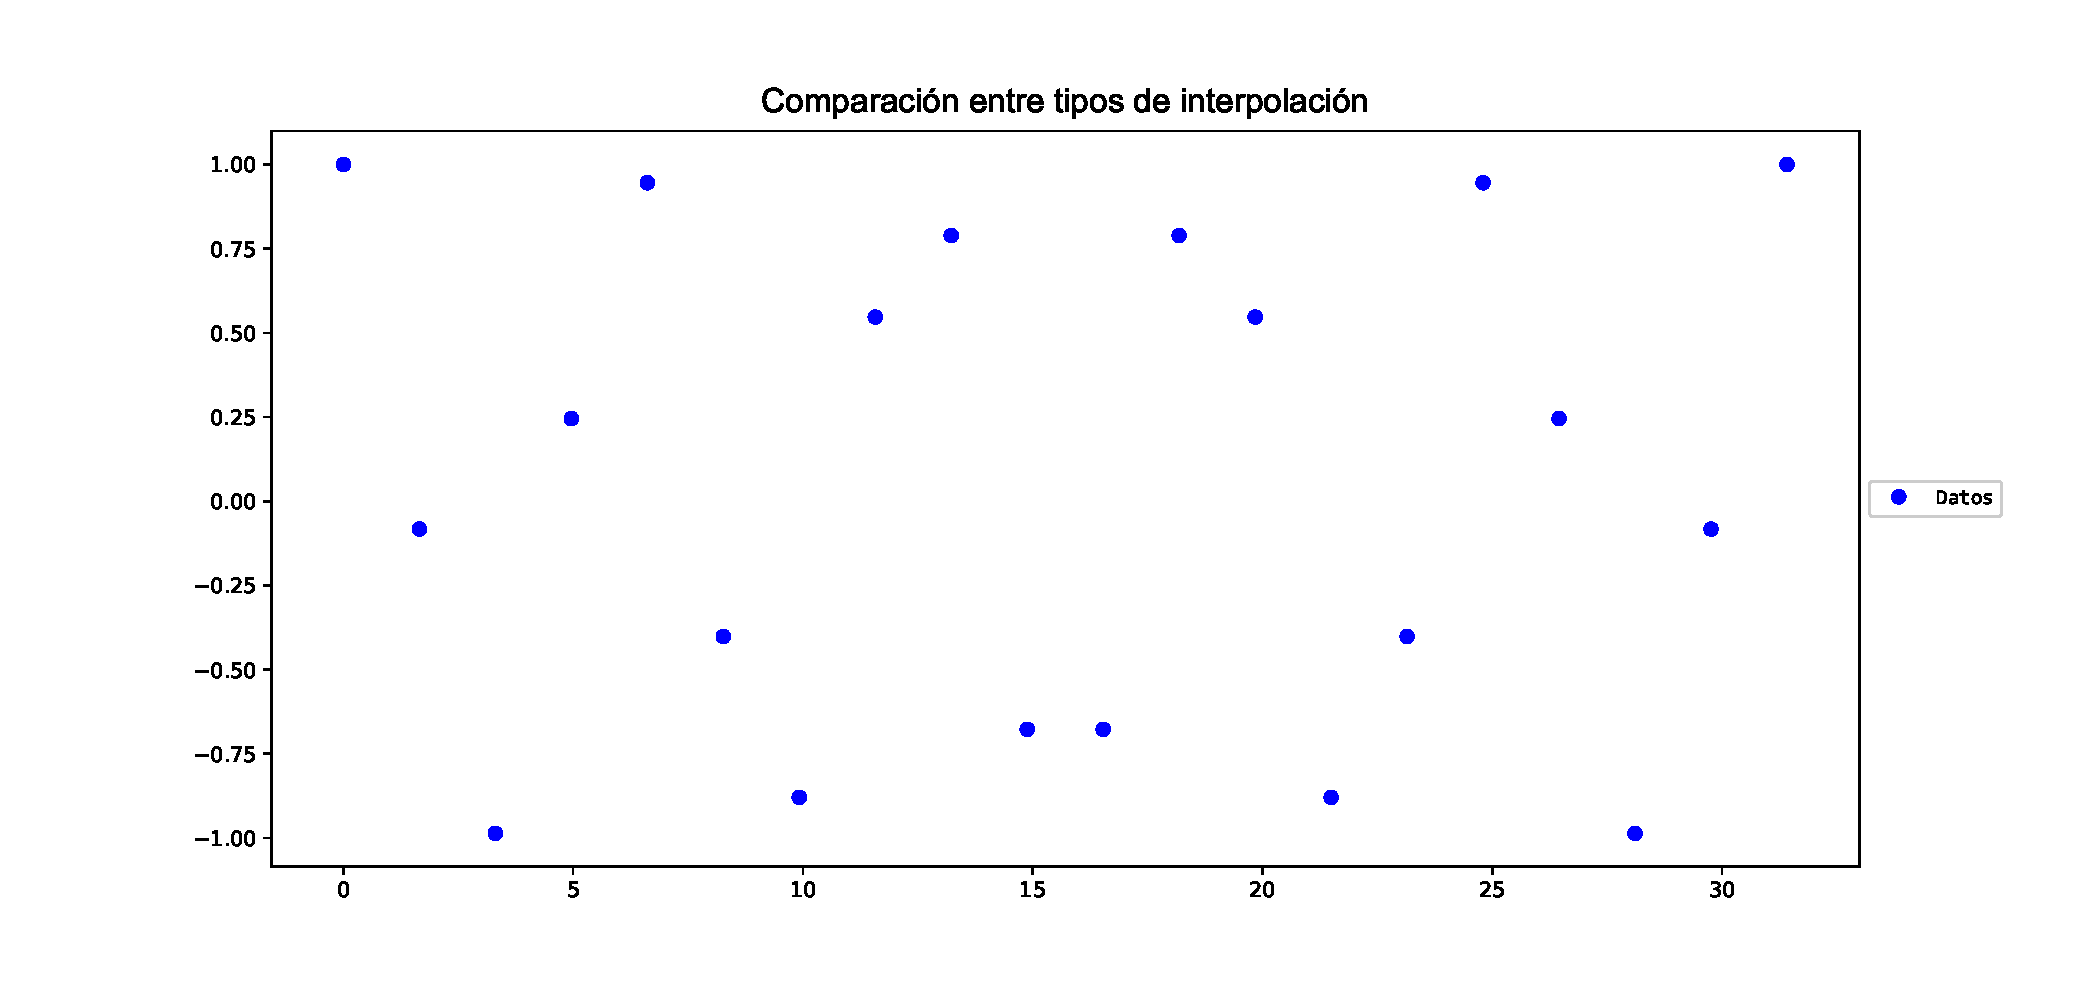
\includegraphics[scale=0.5]{Imagenes/interpolacion_01}
\caption{Datos iniciales con los que vamos a interpolar.}
\end{figure}
\end{frame}
\begin{frame}[allowframebreaks, fragile]
\frametitle{Se interpolan los datos}
\begin{lstlisting}[caption=Cambiando el tipo de interpolación, style= FormattedNumber, basicstyle=\linespread{0.9}\ttfamily=\small, columns=fullflexible]
# Se interpolan los datos

fl = interp1d(x, y, kind='linear')

fq = interp1d(x, y, kind='quadratic')

# x.min and x.max se usan para asegurar que no
# nos salimos del intervalo de interpolacion

xint = np.linspace(x.min(), x.max(), 1000)

yintl = fl(xint)

yintq = fq(xint)

#para graficar

plt.plot(xint, yintl, label='Lineal')

plt.plot(xint, yintq, label='Cuadratica')

plt.legend(loc=1)
plt.show()
\end{lstlisting}
\end{frame}
\begin{frame}
\frametitle{Interpolación lineal}
\begin{figure}
%\centering
\hspace*{-0.2cm}\includegraphics[scale=0.5]{Imagenes/interpolacion_02}
\caption{La función que se obtiene con una interpolación lineal.}
\end{figure}
\end{frame}
\begin{frame}
\frametitle{Interpolación cuadŕatica}
\begin{figure}
%\centering
\hspace*{-0.2cm}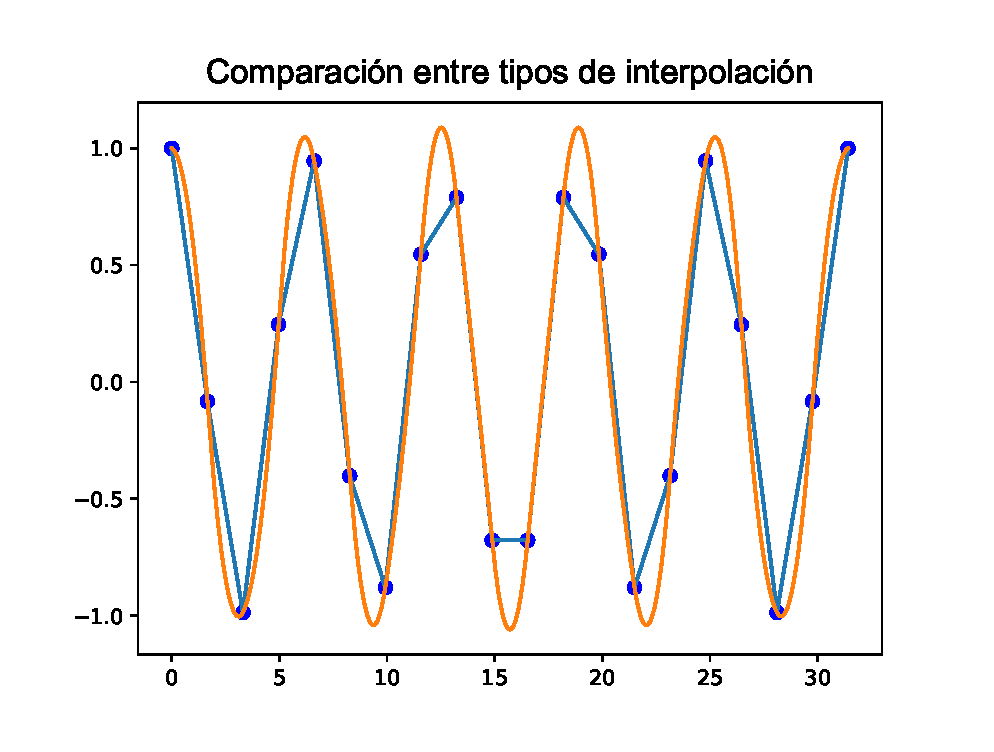
\includegraphics[scale=0.5]{Imagenes/interpolacion_03b}
\caption{La función que se obtiene con una interpolación cúbica.}
\end{figure}
\end{frame}
\subsection{La función \texttt{sinc(x)}}
\begin{frame}
\frametitle{Veamos otro ejemplo: función \azulfuerte{\texttt{sinc(x)}}}
Utilizaremos la función \azulfuerte{\texttt{sinc(x)}} que está contenida dentro de la librería \azulfuerte{\texttt{numpy}}.
\\
\bigskip
La función \azulfuerte{\texttt{sinc(x)}}, también llamada \enquote{función de muestreo}, es una función que se encuentra comúnmente de las teorías de procesamiento de señales y de las transformadas de Fourier.
\end{frame}
\begin{frame}
\frametitle{Función seno cardinal}
El nombre completo de la función es \enquote{seno cardinal}, pero es comúnmente referido por su abreviatura, \enquote{sinc}.
\\
\bigskip
Se define como
\[ sinc(x) = \begin{cases}
1 & \mbox{para } x = 0 \\
\dfrac{\sin x}{x} & \mbox{para cualquier otro valor} \end{cases} \]
\end{frame}
\begin{frame}[fragile]
\frametitle{Generamos algunos datos con \azulfuerte{\texttt{sinc(x)} }}
En el ejercicio vamos a generar un conjunto de datos aleatorio y se van a sumar a los valores de la función \texttt{sinc(x)}, de tal manera que representarían los datos experimentales.
\end{frame}
\begin{frame}[allowframebreaks, fragile]
\frametitle{Código con \python}
\begin{lstlisting}[caption= Datos iniciales para la comparación, style= FormattedNumber, basicstyle=\linespread{0.9}\ttfamily=\small, columns=fullflexible]
import numpy as np
import matplotlib.pyplot as plt

x = np.linspace(-18, 18, 36)

ruido = 0.1 * np.random.random(len(x))
senal = np.sinc(x) + ruido

interpretada = interpolate.interp1d(x, senal)

x2 = np.linspace(-18, 18, 180)
y = interpretada(x2)

cubica = interpolate.interp1d(x, senal, kind="cubic")
y2 = cubica(x2)
\end{lstlisting}
\end{frame}
\begin{frame}
\frametitle{Datos con la señal de muestreo}
\begin{figure}
%\centering
\includegraphics[scale=0.65]{Imagenes/Interpolacion_sinc_01}
\end{figure}
\end{frame}
\begin{frame}
\frametitle{Función con interpolación lineal}
\begin{figure}
%\centering
\includegraphics[scale=0.55]{Imagenes/Interpolacion_sinc_02}
\caption{La función no pasa por todos los puntos aleatorios.}
\end{figure}
\end{frame}
\begin{frame}
\frametitle{Funciones lineal y cúbica}
\begin{figure}
%\centering
\includegraphics[scale=0.55]{Imagenes/Interpolacion_sinc_03}
\caption{Se mejora la aproximación con la interp. cúbica.}
\end{figure}
\end{frame}
\subsection{Características de la interpolación}
\begin{frame}
\frametitle{Más sobre la interpolación.}
Es posible reconocer algunas características generales de la interpolación obtenida en las figuras:
\setbeamercolor{item projected}{bg=red!70!black,fg=white}
\setbeamertemplate{enumerate items}[circle]
\begin{enumerate}[<+->]
\item Las funciones de interpolación son continuas.
\item Las funciones de interpolación pasan siempre por los puntos de datos.
\item Una función cuadrática puede dar un ajuste más malo que la interpolación lineal.
\item Aumentar el orden del polinomio no siempre conduce a un mejor ajuste.
\seti
\end{enumerate}
\end{frame}
\begin{frame}
\frametitle{Más sobre la interpolación.}
\setbeamercolor{item projected}{bg=red!70!black,fg=white}
\setbeamertemplate{enumerate items}[circle]
\begin{enumerate}[<+->]
\conti
\item Las funciones de interpolación pueden oscilar drásticamente entre los puntos de datos.
\item El ajuste empeora hacia los extremos del conjunto de datos.
\end{enumerate}
\end{frame}
\begin{frame}
\frametitle{Entonces, ¿qué debo hacer al interpolar mis propios datos?}
El \enquote{spline cúbico} es el caballo de batalla en este terreno.
\\
\bigskip
Como se puede ver en la siguiente figura, proporciona una curva suave que parece ajustarse bien a los datos.
\end{frame}
\begin{frame}
\begin{figure}
\frametitle{Curva con un ajuste suave}
\centering
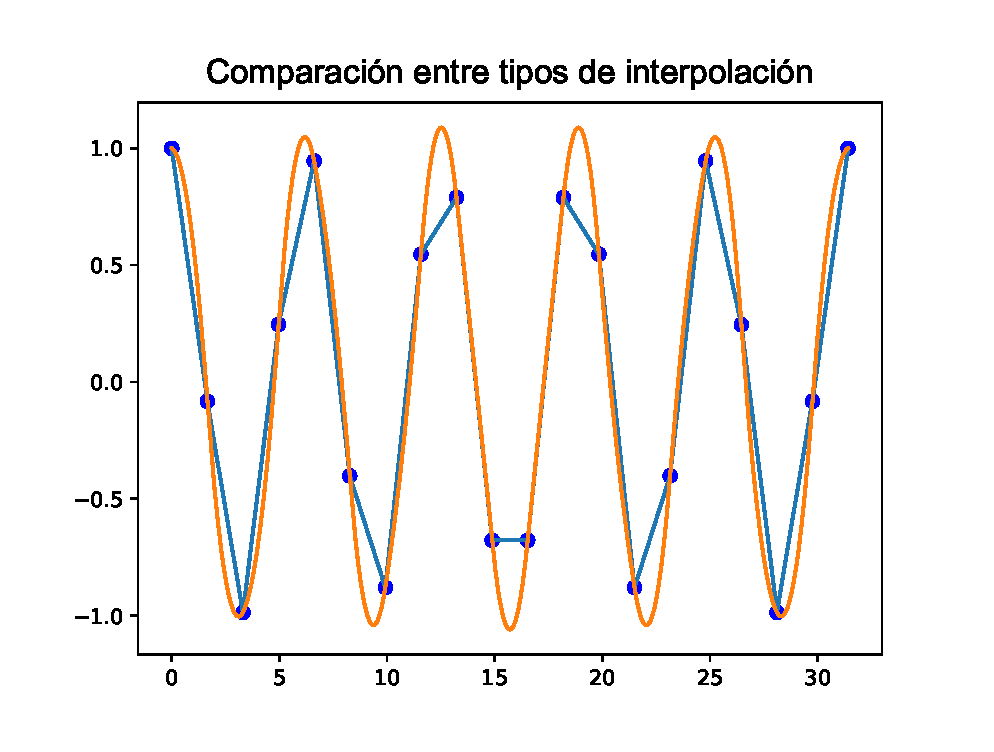
\includegraphics[scale=0.4]{Imagenes/interpolacion_03b}
\end{figure}
\end{frame}
\begin{frame}
\frametitle{La suavidad de la curva}
La suavidad se extiende más allá de lo que se ve en la gráfica: un \enquote{spline cúbico} tiene derivadas primera y segunda continuas.
\\
\bigskip
Esta es una propiedad útil en la física, donde las derivadas primera y segunda son bastante comunes en los análisis teóricos (leyes de Newton, ecuaciones de Maxwell, ecuación de Schröedinger, etc.)
\\
\medskip
\pause
\textcolor{blue}{Una interpolación de spline cúbico es una buena opción en la mayoría de los casos}.
\end{frame}
\begin{frame}
\frametitle{Precaución con las funciones de interpolación}
Precaución: la interpolación y la extrapolación no es lo mismo.
\\
\bigskip
Una buena función de interpolación puede ser una aproximación muy mala fuera del conjunto de puntos de datos utilizados. 
\end{frame}
\begin{frame}
\frametitle{Precaución con las funciones de interpolación}
Por esta razón, las funciones generadas por \azulfuerte{\texttt{interp1d (x, y)}} ni siquiera devolverán un número cuando proporcione un valor de la variable independiente fuera del rango del conjunto de datos: se obtiene un \texttt{ValueError} en su lugar.
\end{frame}
\section{Principios de los splines}
\frame{\tableofcontents[currentsection, hideothersubsections]}
\subsection{Fenómeno de Runge}
\begin{frame}
\frametitle{Fenónemo de Runge}
Hasta el momento hemos revisado un par de estrategias para calcular un polinomio que pase por un conjunto de datos $(x_{i}, y_{i})$, pero hay que considerar un efecto importante al respecto: no siempre el mejor polinomio será aquel el de mayor grado $n$.
\end{frame}
\begin{frame}
\frametitle{Gráfica de la función $f(x)$}
Veamos el siguiente ejemplo: sea la función:
\[ f(x) = \dfrac{1}{1 + 25 x^{2}}\]
\begin{figure}
    \centering
    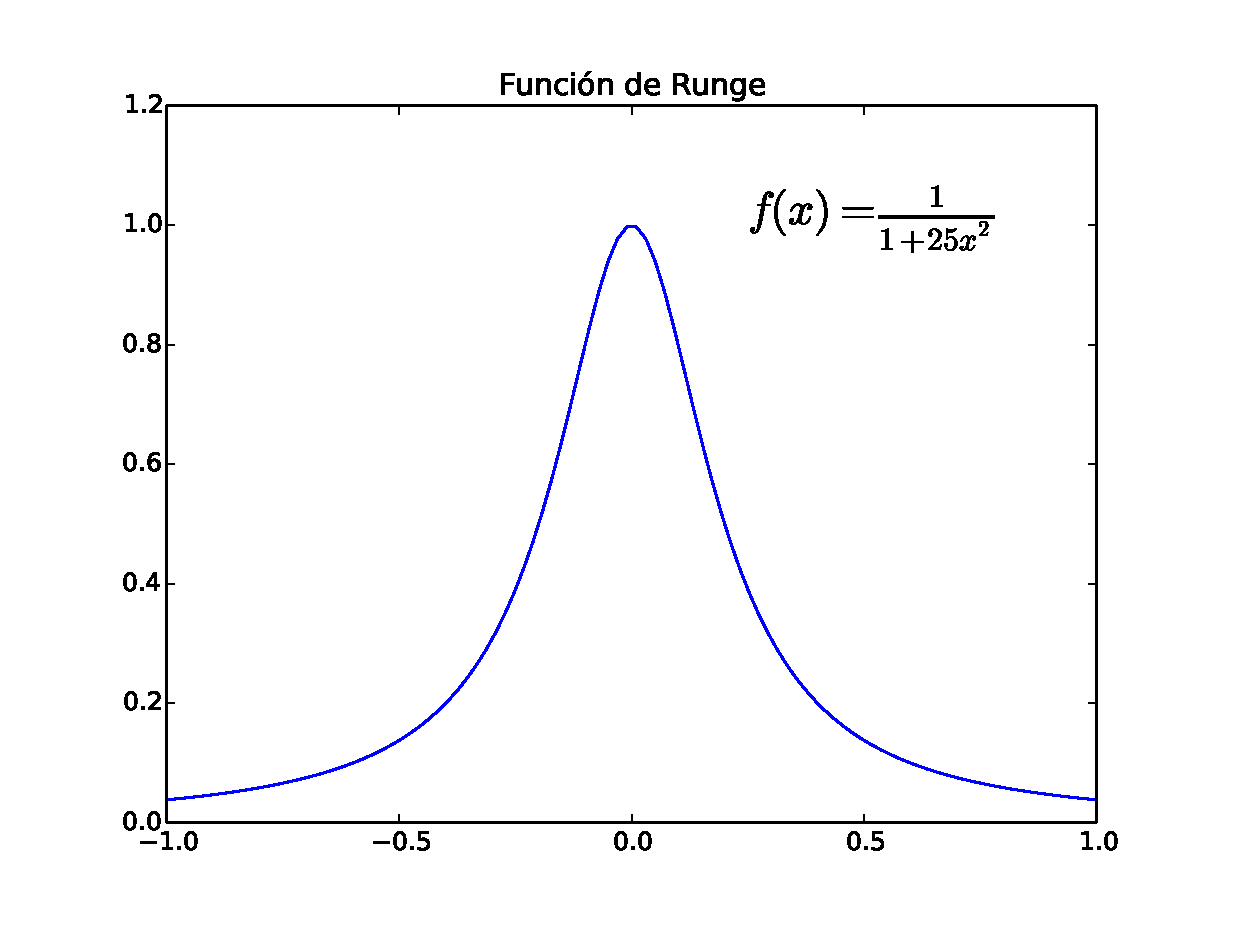
\includegraphics[scale=0.35]{Imagenes/Funcion_Runge_01.eps} 
\end{figure}
\end{frame}
\begin{frame}
\frametitle{Elección de puntos para interpolar}
Elegimos un conjunto aleatorio de puntos a los que vamos a interpolar.
\begin{figure}
    \centering
    \includegraphics[scale=0.4]{Imagenes/Funcion_Runge_02.eps} 
\end{figure}
\end{frame}
\begin{frame}
\frametitle{Interpolación con Lagrange}
Interpolando los puntos con Lagrange.
\begin{figure}
    \centering
    \includegraphics[scale=0.5]{Imagenes/Funcion_Runge_03.eps} 
\end{figure}
\end{frame}
\begin{frame}
\frametitle{¿Qué hacemos al respecto?}
Como hemos visto en la gráfica anterior, la función que resulta del proceso de interpolación \enquote{oscila} a través de los puntos que deseamos interpolar; aquí el caso es que si aumentamos el grado del polinomio, los resultados serán aún más indeseables.
\\
\medskip
\pause
La pregunta obligada es: \textcolor{red}{¿qué podemos hacer para mejorar la interpolación?}
\end{frame}
\subsection{¿Qué es un spline?}
\begin{frame}
\frametitle{¿Qué es un spline?}
En términos nada riguroso, se puede decir que un spline es una función definida por una familia de polinomios \enquote{sociables}.
\\
\bigskip
Donde el término sociable se usa para indicar que los polinomios que constituyen una función spline, están estrechamente vinculados.
\end{frame}
\begin{frame}
\frametitle{¿Qué es un spline?}
El nombre de \emph{spline}, viene del inglés ya que es un instrumento que utilizaban los ingenieros navales para dibujar curvas suaves, forzadas a pasar por un conjunto de puntos prefijados.
\end{frame}
\begin{frame}
\frametitle{Las tres B's de los splines}
El uso de las funciones splines tiene mucha aceptación y popularidad se deben a tres razones básicas:
\setbeamercolor{item projected}{bg=red!70!black,fg=white}
\setbeamertemplate{enumerate items}[circle]
\begin{enumerate}[<+->]
\item \textbf{Buenos:} Se  pueden usar en la solución de una gran variedad de problemas.
\item \textbf{Bonitos:} La teoría matemática en que se basan es muy simple y a la vez elegante.
\item \textbf{Baratos:} Ya que su cálculo es muy sencillo y económico.
\end{enumerate}
\end{frame}
\subsection{Splines con \python}
\begin{frame}
\frametitle{Manejando splines con \python}
Usaremos la librería \azulfuerte{\texttt{scipy}} que contiene varias funciones con las que ahorramos tiempo para manejar splines y ajustar funciones sociables a un conjunto de datos.
\end{frame}
\begin{frame}
\frametitle{Manejando splines con \python}
No está de más que revises la teoría al respecto, en la mayoría de los libros de análisis numérico, podrás encontrar la construcción matemática y formal de los splines.
\end{frame}
\begin{frame}
\frametitle{Funciones para los splines}
Necesitaremos de dos funciones para el uso de splines con \python contenidos en la libería: \azulfuerte{\texttt{scipy.interpolate}}, las cuales son:
\end{frame}
\begin{frame}
\frametitle{La función \azulfuerte{\texttt{splrep}}}
\azulfuerte{\texttt{splrep}}: Calcula el spline básico (B-spline) para una curva 1-D.
\\
\medskip
Dados un conjunto de puntos $(x[i],y[i])$ determina una aproximación con un spline suave de grado $k$ en el intervalo $x_{b} \leq x \leq x_{e}$.
\\
\medskip
En caso de que no se proporcione el intervalo, se toma como tal, los valores $x[0]$ y $x[-1]$
\end{frame}
\begin{frame}[fragile]
\frametitle{Argumentos de la función \azulfuerte{\texttt{splrep}}}
Tomamos la función de la librería \azulfuerte{\texttt{scipy.interpolate}}, la función opera de la siguiente manera:
\fontsize{12}{12}\selectfont
\\
\bigskip
\azulfuerte{\texttt{splrep}}\texttt{(x, y, xb=None, xe=None, k=3 [, otros argumentos])}
\\
\bigskip
\fontsize{14}{14}\selectfont
donde $k$ es el grado de ajuste del spline. Se recomienda utilizar splines cúbicos.
\end{frame}
\begin{frame}
\frametitle{Lo que devuelve \azulfuerte{\texttt{splrep}}}
La función devuelve lo siguiente:
\\
\bigskip
\azulfuerte{\texttt{tck}} : una tupla.
\\
\bigskip
La tupla \azulfuerte{\texttt{(t,c,k)}} contiene el vector de puntos (knots), los coeficientes del B-spline, y el grado del spline.
\end{frame}
\begin{frame}
\frametitle{La función \azulfuerte{\texttt{splev}}}
\azulfuerte{\texttt{splev}}: Evalúa un B-spline o sus derivadas.
\\
\bigskip
Dados los nodos y coeficientes de un B-spline, calcula el valor del polinomio suave y sus derivadas.
\end{frame}
\begin{frame}
\frametitle{Argumentos de la función}
La función opera con los siguientes argumentos (revisa la documentación para obtener más información de los argumentos opcionales)
\\
\bigskip
\azulfuerte{\texttt{splev}} \texttt{(x, tck)}
\end{frame}
\begin{frame}
\frametitle{Argumentos de la función}
\azulfuerte{\texttt{splev}} \texttt{(x, tck)}
\\
\bigskip
donde:
\\
\medskip
$x$ : Es un arreglo de puntos en donde se evalúa el spline suavizado o sus derivadas.
\\
\medskip
$tck$ : Es una tupla de 3 elementos o un objeto B-Spline. Si es la tupla, debe de ser la secuencia que devuelve \azulfuerte{\texttt{splrep}}, que contiene los nodos, los coeficientes y el grado del spline.
\end{frame}
\begin{frame}
\frametitle{Lo que devuelve \azulfuerte{\texttt{splev}}}
\azulfuerte{\texttt{y}} : un n-arreglo o lista de n-arreglos.
\\
\bigskip
Es un arreglo de valores que representan la función spline evaluada en los puntos $x$. Si $tck$ se proporcionó a partir de la función \azulfuerte{\texttt{splrep}}, entonces es la lista de arreglos que representan la curva en el n-espacio dimensional.
\end{frame}
\begin{frame}
\frametitle{La función de Runge y los splines}
Usaremos las dos funciones mencionada para evaluar splines cúbicos como aproximación para la función Runge.
\\
\bigskip
Se cambia el número de puntos $n$ como intervalo para la aproximación.
\end{frame}
\begin{frame}[allowframebreaks, fragile]
\frametitle{Código}
\begin{lstlisting}[caption=Código completo, style= FormattedNumber, basicstyle=\linespread{1.1}\ttfamily=\small, columns=fullflexible]
import matplotlib.pyplot as plt
import scipy.interpolate as si
from numpy import linspace

x = linspace(-1, 1, 100)
y = 1./(1 + 25 * x**2)

def trazadorcub(n):
    xi = linspace(-1, 1, n)
    yi = 1./(1 + 25 * xi**2)
    tck = si.splrep(xi, yi)
    return tck

tck = trazadorcub(8)
ys_8_ = si.splev(x, tck)

tck = trazadorcub(12)
ys_12_ = si.splev(x, tck)

plt.plot(x, y, label='Funcion Runge')
plt.plot(x, ys_8_,'+g-', label='n=8')
plt.plot(x, ys_12_,'+r-',label ='n=12')
plt.legend(loc='best')
plt.title('Interpolacion con splines cubicos')
plt.ylim(-0.2, 1.2)
plt.show()
\end{lstlisting}
\end{frame}
\begin{frame}
\setbeamerfont{caption}{size=\scriptsize}
\begin{figure}
    \centering
    \includegraphics[scale=0.6]{Imagenes/Splines_Runge_04}
    \caption{Al aumentar el número de puntos en el arreglo para la función \azulfuerte{\texttt{splrep}}, mejora la aproximación con el spline cúbico.}
\end{figure}
\end{frame}
}
\end{document}
